\chapter{The Dynamics View}

\begin{goals}
\begin{itemize}
    \item Understand how training dynamics affect what networks learn
    \item Survey NTK, implicit regularization, and double descent
    \item See what dynamics tells us about architecture
\end{itemize}
\end{goals}

\section{The Core Idea}

The final network depends not just on architecture, but on how training unfolds.

\begin{intuition}
Two networks with identical architectures, trained differently, can learn different functions.
\begin{itemize}
    \item Different initializations $\to$ different solutions
    \item Different optimizers $\to$ different implicit biases
    \item Different stopping times $\to$ different generalization
\end{itemize}
\end{intuition}

The dynamics of gradient descent itself shapes the solution.

\section{Neural Tangent Kernel}

\subsection{The Discovery}

Jacot et al. (2018) showed: in the infinite-width limit, neural network training simplifies dramatically.

\begin{definition}[Neural Tangent Kernel]
For a network $f_\theta(x)$, the NTK is:
\[
K(x, x') = \left\langle \nabla_\theta f_\theta(x), \nabla_\theta f_\theta(x') \right\rangle
\]
\end{definition}

\begin{theorem}[Jacot et al.]
As width $\to \infty$:
\begin{enumerate}
    \item The NTK converges to a deterministic limit
    \item The NTK stays constant during training
    \item Training reduces to kernel regression with this fixed kernel
\end{enumerate}
\end{theorem}

\subsection{Implications}

In this ``lazy training'' regime:
\begin{itemize}
    \item Dynamics are linear (in function space)
    \item Convergence to global minimum is guaranteed
    \item The kernel is determined by architecture alone
\end{itemize}

\begin{keyinsight}
NTK says: for infinite-width networks, architecture determines a kernel, and training is just kernel regression.
\end{keyinsight}

\subsection{Limitations}

\begin{warning}
The NTK regime \textbf{cannot do feature learning}.

Weights stay near initialization. The network doesn't learn new representations — it just fits with the initial (random) features.
\end{warning}

Real networks (finite width, trained long enough) leave the lazy regime and learn features. NTK doesn't capture this.

\begin{center}
\begin{tabular}{lll}
\textbf{Regime} & \textbf{Weights move?} & \textbf{Features learned?} \\
\hline
Lazy (NTK) & Little & No \\
Feature learning & A lot & Yes \\
\end{tabular}
\end{center}

\section{Implicit Regularization}

\subsection{The Puzzle}

Neural networks generalize well even when:
\begin{itemize}
    \item They have more parameters than data points
    \item No explicit regularization (no L1/L2)
    \item They can perfectly fit random labels
\end{itemize}

Why don't they overfit?

\subsection{The Answer: SGD Has Preferences}

Gradient descent doesn't just find \emph{any} solution — it finds particular ones.

\begin{definition}[Implicit Regularization]
The bias of gradient descent toward certain solutions, independent of explicit regularization.
\end{definition}

\begin{example}[Linear Networks]
For linear networks (no activation), gradient descent converges to the minimum-norm solution:
\[
\min_\theta \|w\|_2 \quad \text{subject to fitting the data}
\]
\end{example}

\begin{example}[Matrix Factorization]
For $W = UV^\top$ (deep linear networks), gradient descent biases toward low-rank solutions.
\end{example}

\subsection{Architecture Affects Implicit Bias}

Different architectures induce different implicit regularizers.

\begin{itemize}
    \item Deeper networks $\to$ stronger low-rank bias
    \item Initialization scale affects bias (small $\to$ L1-like, large $\to$ L2-like)
    \item Activation function matters
\end{itemize}

\begin{warning}
Most rigorous results are for linear networks.

Nonlinear networks are much harder to analyze.
\end{warning}

\section{Double Descent}

\subsection{The Phenomenon}

Classical wisdom: more parameters $\to$ more overfitting.

Modern observation: it's more complicated.

\begin{definition}[Double Descent]
As model complexity increases:
\begin{enumerate}
    \item Test error decreases (underfitting regime)
    \item Test error increases (overfitting regime)
    \item Test error decreases again (interpolating regime)
\end{enumerate}
\end{definition}

The second descent happens when the model is large enough to interpolate (fit training data exactly).

\subsection{The Interpolation Threshold}

The peak of the ``U'' occurs near the \textbf{interpolation threshold}: where \# parameters $\approx$ \# training samples.

\begin{center}
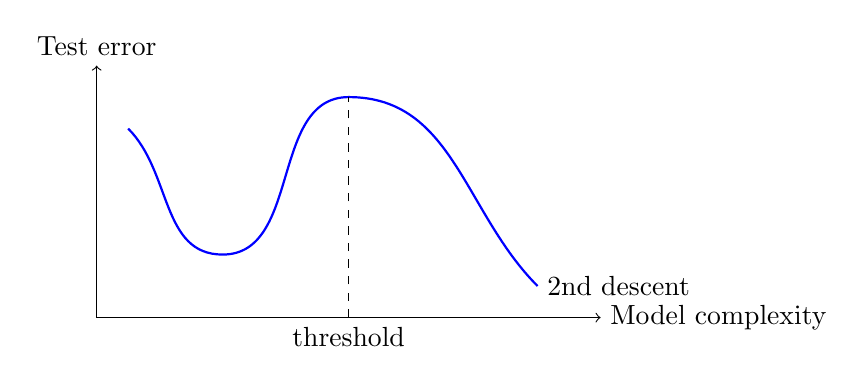
\begin{tikzpicture}[scale=0.8]
\draw[->] (0,0) -- (8,0) node[right] {Model complexity};
\draw[->] (0,0) -- (0,4) node[above] {Test error};
\draw[thick, blue] (0.5,3) to[out=-45,in=180] (2,1) to[out=0,in=180] (4,3.5) to[out=0,in=135] (7,0.5);
\draw[dashed] (4,0) -- (4,3.5);
\node[below] at (4,0) {threshold};
\node[right] at (7,0.5) {2nd descent};
\end{tikzpicture}
\end{center}

\subsection{Implications}

\begin{keyinsight}
``Bigger is better'' and ``smaller is better'' are both wrong.

The relationship between size and generalization is non-monotonic.
\end{keyinsight}

For architecture design: you can't just minimize parameters. Sometimes more parameters (in the right regime) generalize better.

\section{What Dynamics Tells Us}

\subsection{Strengths}

\begin{itemize}
    \item \textbf{Explains surprises}: Why overparameterized networks generalize
    \item \textbf{Reveals hidden structure}: Implicit regularization is real
    \item \textbf{Guides practice}: Don't fear the interpolating regime
\end{itemize}

\subsection{Limitations}

\begin{itemize}
    \item \textbf{Descriptive, not prescriptive}: Explains what happens, not what to do
    \item \textbf{Architecture-specific}: Each architecture has different dynamics
    \item \textbf{Hard to analyze}: Nonlinear dynamics are complex
\end{itemize}

\section{Relevance to Our Question}

Dynamics tells us: the path of optimization matters, not just the endpoint.

For learning logical structures:
\begin{itemize}
    \item The semiring relaxation creates a particular loss landscape
    \item Gradient descent will have some implicit bias on this landscape
    \item We don't yet know what that bias is
\end{itemize}

\begin{keyinsight}
We've focused on ``what to parameterize'' (architecture). Dynamics says ``how you optimize'' also matters.

A full theory of ``learning well'' needs both.
\end{keyinsight}
